\documentclass[conference]{IEEEtran}
\IEEEoverridecommandlockouts
% The preceding line is only needed to identify funding in the first footnote. If that is unneeded, please comment it out.
\usepackage{cite}
\usepackage{amsmath,amssymb,amsfonts}
\usepackage{algorithmic}
\usepackage{graphicx}
\usepackage{textcomp}
\usepackage{xcolor}
\usepackage{hyperref}
\usepackage{float}
\usepackage{minted}



\def\BibTeX{{\rm B\kern-.05em{\sc i\kern-.025em b}\kern-.08em
    T\kern-.1667em\lower.7ex\hbox{E}\kern-.125emX}}
\begin{document}

\title{Aviation Small Language Model \\ Configuration, Training, Inference}

\author{\IEEEauthorblockN{Samrat Kar}
Bangalore, India}

\maketitle

\begin{abstract}
This paper develops a small language model (SLM). Trains it with the Julius Caesar text. And then it uses the it generates new texts based on the knowledge gained form the text. The model parameters are stored for future use and application development. The various fine tuning is done, to improvise the model to reduce overfitting. 
Then the model is trained on Tiny Stories dataset to be able to make the model create legible English sentences. Then it is fine tuned with Aerospace Questions and Answers to make it able to answer on the domain related questions.
\end{abstract}

\section{Introduction}
The code implements the multi-head attention mechanism using Transformer architecture. The Julius Caesar text is taken from Project Gutenberg and it is used to train the model. 

\section{Steps to build the SLM}
\begin{itemize}
    \item Get the dataset and 
    \item Tokenize the dataset using tiktoken library.
    \item Split the data set into test and train and store the data set in a memory-mapped array to avoid RAM overload.
    \item Create input-output batches for the dataset for both test and train split.
    \item Do the layer normalization for regularization
    \item Compute \textbf{Context Matrix} 
    \begin{itemize}
        \item Compute \textbf{Causal Attention Score} Matrix (MHA: Multi-head attention)
        \begin{itemize}
            \item initialize the $W_q, W_k, W_v$ matrix
            \item Query Matrix $Q = X \times W_q$ (X = input matrix)
            \item Key Matrix $K =  X \times W_k$ 
            \item Value Matrix $V = X \times W_v$
            \item Attention score $att = (Q \times K^T)/ \sqrt{dim}$
            \item Masking attention score by $-\infty$ on the upper diagonal of the Attention Score.
            \item $att = softmax(att \ score)$
            \item self attention dropout
        \end{itemize}
        \item \textbf{Context Matrix} = $y = att \times V$
    \end{itemize}
    \item Dropout on \textbf{Context matrix} 
    \item Pass context matrix to \textbf{Multi-layer perceptron feedforward neural network. (MLH)} with GELU activation function to train the model
\end{itemize}

\section{Codebase}

\href{https://colab.research.google.com/github/samratkar/samratkar.github.io/blob/main/_posts/concepts/genai/notes-codes/slm-from-scratch/slm-jc.ipynb}{Working SLM codebase trained on Julius Caesar text}

\section{Dataset}

\href{https://www.gutenberg.org/cache/epub/1522/pg1522.txt}{Julius Caesar full text}

\section{Model}

\href{https://huggingface.co/samratkar/slm_julius_caesar}{
  \includegraphics[height=16pt]{hf-jc.png}
}

\section{Baselined Model Config}
\begin{itemize}
    \item learning rate = 1e-4
    \item max iters = 10000
    \item warmup steps = 2000
    \item min lr = 5e-4
    \item eval iters = 500
    \item batch size = 8
    \item block size = 128
    \item vocab size=50257 
    \item block size=128 
    \item number of layers=4 
    \item number of heads=4 
    \item embedding dimension=768 
    \item dropout=0.01 
    \item bias=True
\end{itemize}

\section{baseline loss functions}
\label{baseline}
\begin{figure}[H]
    \centering
    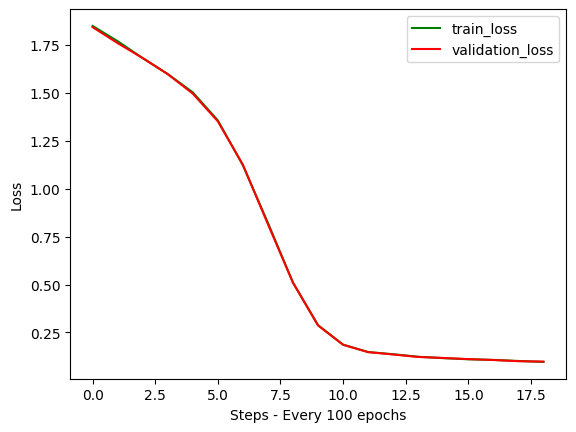
\includegraphics[width=1\linewidth]{10kep.png}
    \caption{baselined losses with 10,000 epochs}
    \label{fig:baselined losses with 10,000 epochs}
\end{figure}

\section{Inference output}
\subsection{Input text} 
"Friends, Romans, countrymen"
\subsection{Output text} 
Friend, Romans, countrymen tyrant. Sh Shall slaves, Then leave their made. Shall I noounds, Most noble Caesar, eries. Stir not resolved,
I can o’ersway him, weep for I please him come to pieces! Here:
CASSIUS.
I know not think it is but a noble Roman, That himKnow I these fires, why all this.

Why obscurely prey: theirFly, why, this conspirators. You shall sober form of heralds to astonish us.

CASSIUS. You are dull, Casca; and those sparks of life That should be in a Roman you do want, Or else you use not. You look pale and gaze, And put on fear and cast yourself in wonder, To see the strange impatience of the Heavens:But if you would consider the true cause Why all these fires.
\section{Analysis of Loss with epochs}
\subsection{epochs : 500}
The graph for training and validation losses for number of epochs as 500 is shown below. There is a huge gap between validation and training loss. This is due to overfitting. The model has not yet learnt the actual pattern of the data. While training the loss got minimized to less than zero. But while testing with new data, there were huge losses. In the order of 8-10.
\begin{figure}[H]
    \centering
    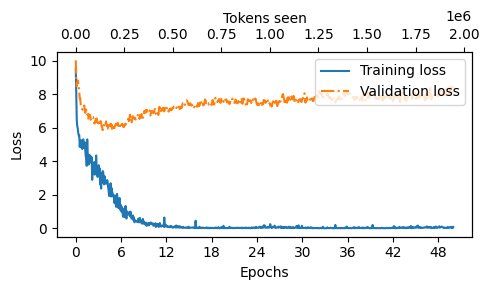
\includegraphics[width=1\linewidth]{training-validation-loss.png}
    \caption{Trg, Test Loss with 500 epochs}
    \label{fig:epoch500}
\end{figure}

\subsection{epochs : 4000}
With increasing epochs from 500 to 4000 the validation and test losses now decrease gradually together and becomes lower than 3.5. The trend of decrease is continuous and throughout the training and validation loss go hand in hand. That shows that the model is not overfitting.
\begin{figure}[H]
    \centering
    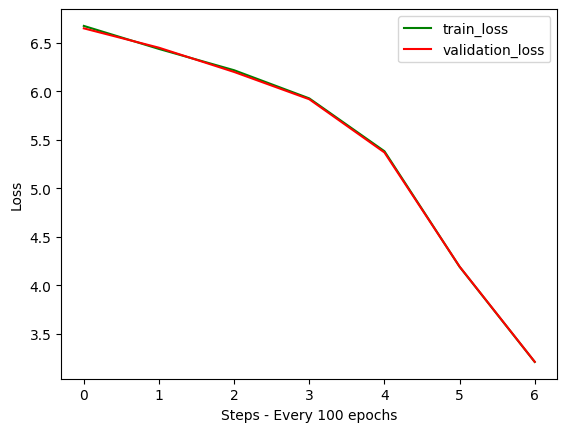
\includegraphics[width=1\linewidth]{4kep.png}
    \caption{Trg, Test Loss}
    \label{fig:epoch4000}
\end{figure}

\subsection{epochs : 10,000}
This is the baselined number of epochs I have for this model. This performance is the best. The loss gradually reduces and both the validation and training losses follow each other. The final loss is of the order 
\begin{figure}[H]
    \centering
    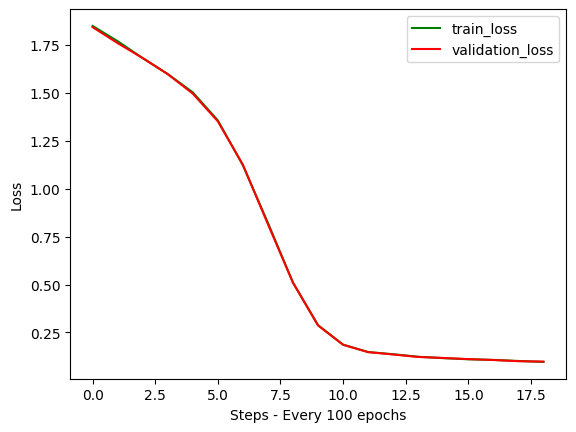
\includegraphics[width=1\linewidth]{10kep.png}
    \caption{Trg, Test Loss}
    \label{fig:epoch10000}
\end{figure}

\subsection{epochs : 20,000}
The more epochs, reduces the loss drastically and it keeps flat at the lowest value. So, going forward, 10K epochs can be considered as the best baseline epochs. Going till 20K is not required.
\begin{figure}[H]
    \centering
    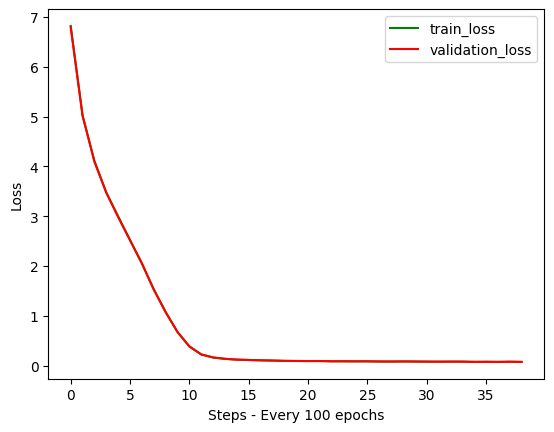
\includegraphics[width=1\linewidth]{20Kep.png}
    \caption{Trg, Test Loss}
    \label{fig:epoch20000}
\end{figure}

\section{Training & validation loss analysis for changing learning rates}
\subsection{Epoch : 10,000, learning rate = 1e-4}
\begin{figure}[H]
    \centering
    \includegraphics[width=1\linewidth]{10Kep.png}
    \caption{Trg, Test Loss, epoch 10K, LR 1e-4}
    \label{fig:epoch}
\end{figure}
\subsection{Inference}
\subsubsection{Input}
"Friends, Romans, countrymen"
\subsubsection{Output}
Friend, Romans, countrymen tyrant. Sh Shall slaves, Then leave their made. Shall I noounds, Most noble Caesar, eries. Stir not resolved,
I can o’ersway him, weep for I please him come to pieces! Here:
CASSIUS.
I know not think it is but a noble Roman, That himKnow I these fires, why all this.

Why obscurely prey: theirFly, why, this conspirators. You shall sober form of heralds to astonish us.

CASSIUS. You are dull, Casca; and those sparks of life That should be in a Roman you do want, Or else you use not. You look pale and gaze, And put on fear and cast yourself in wonder, To see the strange impatience of the Heavens:But if you would consider the true cause Why all these fires.

\subsection{Epoch : 10,000, learning rate = 1e-3}
\begin{figure}[H]
    \centering
    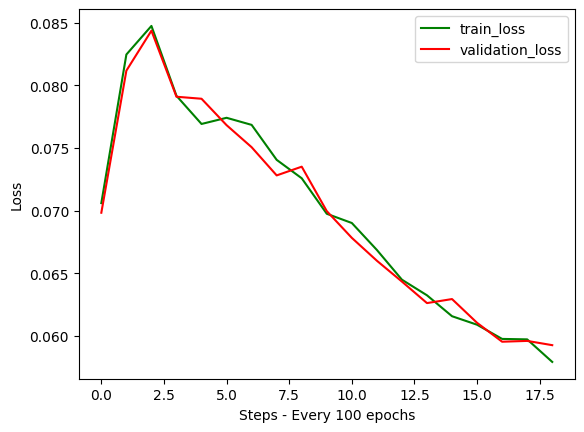
\includegraphics[width=1\linewidth]{lr-1e-3.png}
    \caption{Trg, Test Loss, epoch 10K, LR 1e-3}
    \label{fig:epoch}
\end{figure}
\subsubsection{Input}
"Friends, Romans, countrymen"
\subsubsection{Output}
Friend, Romans, countrymen, And this,The unaccustom’d ope their hearts.It is rage,That unvious Casca or And will 
But when he was no fellow?

BRUTUS.
You; 

OCTAVI know,
As dear abide my right well as you these grief, Whereinna,
As last of him better of this very strong; IUS. Rushing on me, should be not know you? I will please him; PINDAR. What do know you could not, As they do use and keep’d of women;
But keep that which is a fall, Nor for justice?
A man fell. O, coward or a chants.
Thou thrice: Let’d How offer’d, as when Even so appearing to his wife to me, Who, then, as he was a time him

\subsection{Epoch : 10,000, learning rate = 1e-2}
The loss shows a local minima and then it increases. This learning rate is not good for the global minima
\begin{figure}[H]
    \centering
    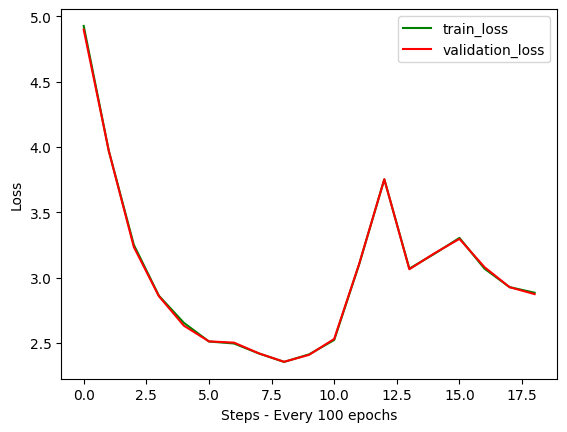
\includegraphics[width=1\linewidth]{lr-1e-2.png}
    \caption{Trg, Test Loss, epoch 10K, LR 1e-2}
    \label{fig:epoch}
\end{figure}
\subsubsection{Input}
"Friends, Romans, countrymen"
\subsubsection{Output}
Friend, Romans, countrymen my legions:
I have to know of some talk more than you are not.
It which we are; is paid in the world at a
There by you of Philippi.
Who you have you demand.
Do;I hopeIt, Else who you shall say you by this? I have removed, including Or) not” or forth by following which you have removed, this work the permission and you comply, the Project Gutenberg™ License included through this night; What. Do, you shall have citizen upon the market-place; are save, fates with the manager of earth render him, displayed, for fates with this work in many hearts, much you provide a king; forth, perform” For You may become the work from him to other work for someone to sleep’d them
Why he which“Break up. There is for someone to hear. If you know of men

\section{Training \& validation loss analysis for changing number of layers}
\subsection{Epoch : 10,000 ; learning rate = 1e-4 ; number of layers = 4}
same as the baseline results of the model in \textbf{Section :} \ref{baseline}

\subsection{Epoch : 10,000 ; learning rate = 1e-4 ; number of layers = 1}
The losses are gradually decreasing to the order of 0.04
\begin{figure}[H]
    \centering
    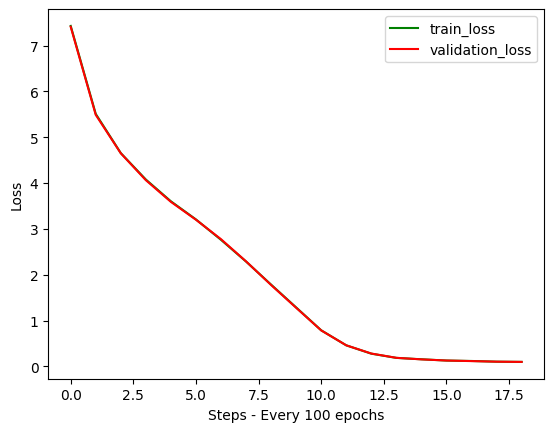
\includegraphics[width=1\linewidth]{1layer.png}
    \caption{Trg, Test Loss, epoch 10K, 1 layer}
    \label{fig:epoch}
\end{figure}
\subsubsection{Input}
"Friends, Romans, countrymen"
\subsubsection{Output}
Friend, Romans, countrymen
HereHis ’BER creditrousED,To held the body,defect in hisopt hands,
with the law of and official page at required to maintaining tax treatment of donations fromwith the souls, and those impatience of the PG search our;  TITINIUS. MESSALA. Will you go see you harm spark,And Shakespeare I elect to provide, in pit, let me.

CASSIUS.
And let us swear our resolution.

BRUTUS.
No, not an office for a fray, And so, I will strive with the have things impossible, Yea, get the better of the better of them.

BRUTUS. A piece of work that will make sick men whole. 

LIGARIUS.
But are not some whole that we must make sick?

BRUTUS.
That must we.

\subsection{Epoch : 10,000 ; learning rate = 1e-4 ; number of layers = 3}
The profile of the loss curves remain similar
\begin{figure}[H]
    \centering
    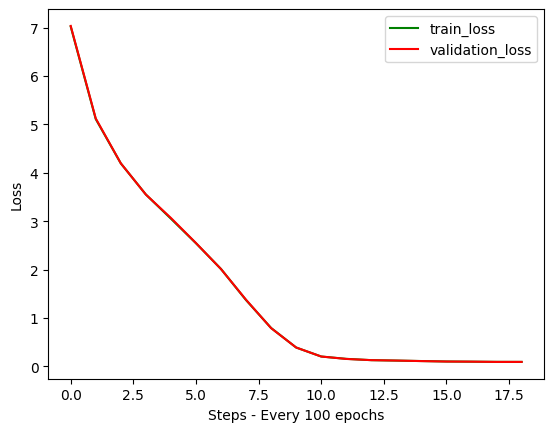
\includegraphics[width=1\linewidth]{3layer.png}
    \caption{Trg, Test Loss, epoch 10K, 3 layer}
    \label{fig:epoch}
\end{figure}
\subsubsection{Input}
"Friends, Romans, countrymen"
\subsubsection{Output}
Friend, Romans, countrymen Project Gutenberg mission of Project Gutenberg
Archman you Live a soldier,
Thespeechless prisoner.

ANTONY.
 Greek. • You provide, in accordance with paragraph 1.F.3, a full refund of      distribution of or providing • You provide, in accordance with paragraph 1.F.3, a full refund of any money paid for a work or a replacement copy, if a defect in the  works.• You comply with all other terms of thisigg rejoice? BUT NOT • You comply, receipt of the work.• You comply with all other terms of this agreement for free    distribution of Project Gutenberg™ works.

 \subsection{Epoch : 10,000 ; learning rate = 1e-4 ; number of layers = 5}
 The profile of the loss curves remain similar
\begin{figure}[H]
    \centering
    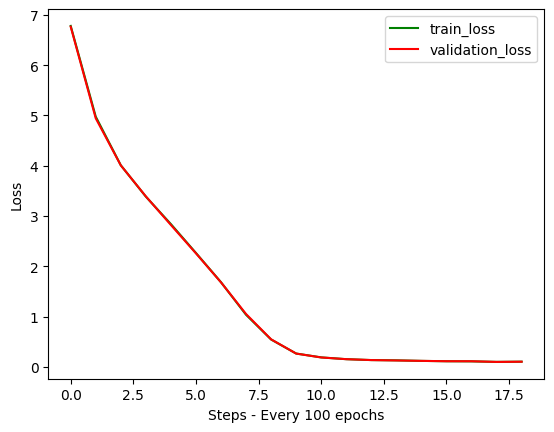
\includegraphics[width=1\linewidth]{5layer.png}
    \caption{Trg, Test Loss, epoch 10K, 5 layer}
    \label{fig:epoch}
\end{figure}
\subsubsection{Input}
"Friends, Romans, countrymen"
\subsubsection{Output}
Friend, Romans, countrymen,—
Which appear, off cried, minds stay’d to poor Brutus,
ber, orearilius,
Not littleKnow you depart, as you received the strength of others.

BRUTUS.
Therein our letters, do not well agree.
Mine speak of seventy Senators that died
By their proscriptions, Cicero being one.

CASSIUS.
Cicero one!

C improve them, may:
Then lest that the day break here womanish speaksby
CASCA.
Indeed, they say the senators tomorrow
MeusFUN neigh, and dying men did incertain to establish Caesar
My format withfrom even into the Project Gutenberg™
omes Caesar with a fever when he was in Spain,
And when the fit was on him I did mark
And when the fit was on him I did mark
How he did shake: ’tis true, this god did shake:

\subsection{Epoch : 5,000 ; learning rate = 1e-4 ; number of layers = 7}
Reducing the epochs to 5K, as the losses are less. The loss remains in the same order
Epoch 4500: train loss 0.2312, val loss 0.2319
The current learning rate: 0.00048
\begin{figure}[H]
    \centering
    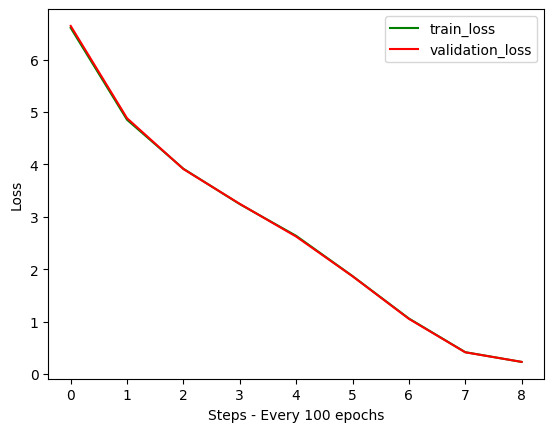
\includegraphics[width=1\linewidth]{7layer5kep.png}
    \caption{Trg, Test Loss, epoch 5K, 7 layer}
    \label{fig:epoch}
\end{figure}
\subsubsection{Input}
"Friends, Romans, countrymen"
\subsubsection{Output}
Friend, Romans, countrymen, that theThings along,CAESAR.
cy fellowman!

CASSIUS.
Goodnight then.
Fulfill your brother, traitors, and UT 84 j pleasingHe wheels?
 letheeunt we say?

CASCA.
O once forms, I am.

Sink in the calendar, ho!bonius. Soul of Rome.rostrum. Alarum. Enter Brutus.

BRUTUS.
Peace! Antony, boy, a table.

ANTONY.
These knew the images, March is unCARPINDARUS.Above.Titinius is a Shall dear brother Cassius! I know some immediate legalize PROJECT GUTUS. They pardon. O, this sink!
I, shame! I do not slept. at Rocket, And entPopilius

\subsection{Epoch : 5,000 ; learning rate = 1e-4 ; number of layers = 12}
Epoch 4500: train loss 0.2377, val loss 0.2393
The current learning rate: 0.00048
Loss remains same as above.
\begin{figure}[H]
    \centering
    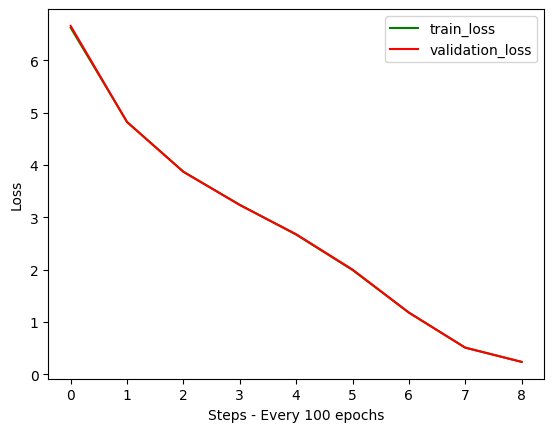
\includegraphics[width=1\linewidth]{12layer5kep.png}
    \caption{Trg, Test Loss, epoch 5K, 12 layer}
    \label{fig:epoch}
\end{figure}
\subsubsection{Input}
"Friends, Romans, countrymen"
\subsubsection{Output}
Friend, Romans, countrymen, lies up their bos make a lamb Yet something leads me.speaks. ign trademark, whilst I cry hand, yea, or a god did love Liter Calphurnia;
 brow, Lucius.

CASSIUS.
Stand fast, their names are fools?

BRUTUS.
Your ear to here again, stand tillie hence,
And then confounded witharius.
ceive a Timelinejay Tank mind inion, Cassius.
But if aellectual property infringement,
triumph.

CASSIUS.
Canst thou art a mace upon my ambition’dler than yourself
And tell me ho!

BRUTUS.
Even so, Cassius, hence, how should I leave anything.

CASSIUS.
Go to, traitors,ella along your recount hereafter. Here’s

BRUTUS.
Come to an itching

\section{Losses trends with varying attention heads}
\subsection{Epoch : 5,000 ; learning rate = 1e-4 ; number of layers = 7 ; number of heads = 1 }
Epoch 4500: train loss 0.1997, val loss 0.1998
The current learning rate: 0.00048
Loss remains same as above.
\begin{figure}[H]
    \centering
    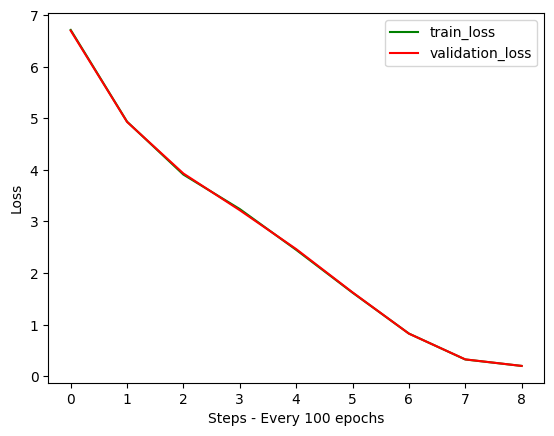
\includegraphics[width=1\linewidth]{7layer1head.png}
    \caption{Trg, Test Loss, epoch 5K, 7 layers 1 head}
    \label{fig:epoch}
\end{figure}
\subsubsection{Input}
"Friends, Romans, countrymen"
\subsubsection{Output}
Friend, Romans, countrymen may himself;
 copying and envy vaccinesKnock within,:

ook it in the Senators,
rose ninth hour, by the user, in thejo within accessible by the United States presently�
         whatsoever. You must gro withholds talk to the uttermost?
CINNA, you thr ours Cassius, and he put it by his hearts,
distribut of this battle brow thinking, he shall lead
For Brutus, to eternal devil,
Are levying powers; we must be whisper
SheChoook it in triumph,
 bade me.
I shall find time,
Only be patient Compliance requirements are not Believe medisposed time.
But-added, and rob the Hybla bees,
Anditating that anybody of thych: security gives demand of describ’d
PROVID speak with the poet,
In theest ready to any majestic world, like
oop then, like

\subsection{Epoch : 5,000 ; learning rate = 1e-4 ; number of layers = 7 ; number of heads = 2}
Epoch 4500: train loss 0.1997, val loss 0.1998
Epoch 3000: train loss 1.7440, val loss 1.7347
The current learning rate: 0.00030
Epoch 3500: train loss 0.9145, val loss 0.9197
The current learning rate: 0.00038
Epoch 4000: train loss 0.3628, val loss 0.3656
The current learning rate: 0.00044
Epoch 4500: train loss 0.2016, val loss 0.2008
The current learning rate: 0.00048
Epoch 4999: train loss 0.2016, val loss 0.2008
The current learning rate: 0.00050
\begin{figure}[H]
    \centering
    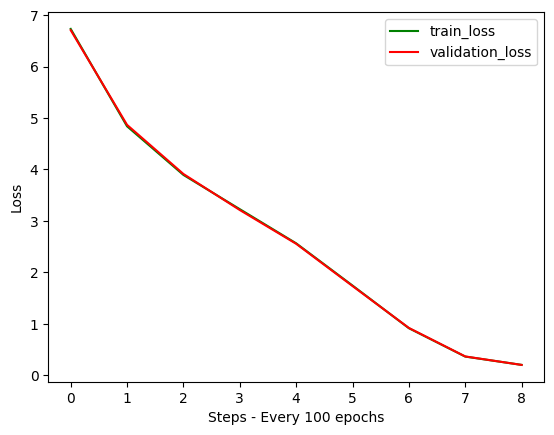
\includegraphics[width=1\linewidth]{7layer2heads.png}
    \caption{Trg, Test Loss, epoch 5K, 7 layers 2 heads}
    \label{fig:epoch}
\end{figure}
\subsubsection{Input}
"Friends, Romans, countrymen"
\subsubsection{Output}
Friend, Romans, countrymen, for theM consent to the readable by the Comes
Fly, and to the streets of the Project Gutenberg™Gutenberg™ eBooks;
That should be in theproduction, savage thusGrant.
So get hold his purpose is oft as to be fear’d to be unnumber’d all;
For if you should be What’dExe
 they may one doth wish
That made wrong’d you and I will look available for briefly,
house, like catching; for my menel;
And I will not disclose ’tis down, good sword,
I abide thisies

CASSIUS.
Am I notwell the feet;
And I tyrants do find it now.
Asinct deductible to their reasons said through Caesar hath whelius.

CAESAR.
What is’s all fool day!
What change, I will turn read gaze,
And

\subsection{Epoch : 5,000 ; learning rate = 1e-4 ; number of layers = 7 ; number of heads = 4}
Epoch 2000: train loss 3.2573, val loss 3.2599
The current learning rate: 0.00016
Epoch 2500: train loss 2.6309, val loss 2.6175
The current learning rate: 0.00022
Epoch 3000: train loss 1.8860, val loss 1.8803
The current learning rate: 0.00030
Epoch 3500: train loss 1.0726, val loss 1.0635
The current learning rate: 0.00038
Epoch 4000: train loss 0.4066, val loss 0.4046
The current learning rate: 0.00044
Epoch 4500: train loss 0.2245, val loss 0.2278
The current learning rate: 0.00048
Epoch 4999: train loss 0.2245, val loss 0.2278
The current learning rate: 0.00050
\begin{figure}[H]
    \centering
    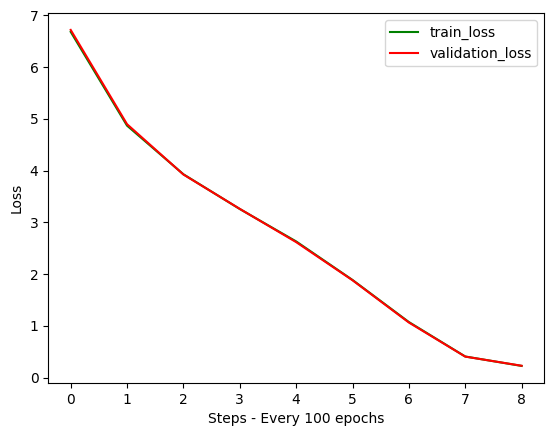
\includegraphics[width=1\linewidth]{7layer4heads.png}
    \caption{Trg, Test Loss, epoch 5K, 7 layers 4 heads}
    \label{fig:epoch}
\end{figure}
\subsubsection{Input}
"Friends, Romans, countrymen"
\subsubsection{Output}
Friend, Romans, countrymen, for theM consent to the readable by the Comes
Fly, and to the streets of the Project Gutenberg™Gutenberg™ eBooks;
That should be in theproduction, savage thusGrant.
So get hold his purpose is oft as to be fear’d to be unnumber’d all;
For if you should be What’dExe
 they may one doth wish
That made wrong’d you and I will look available for briefly,
house, like catching; for my menel;
And I will not disclose ’tis down, good sword,
I abide thisies.

CASSIUS.
Am I notwell the feet;
And I tyrants do find it now.
Asinct deductible to their reasons said through Caesar hath whelius.

CAESAR.
What is’s all fool day!
What change, I will turn read gaze,
And

\subsection{Epoch : 5,000 ; learning rate = 1e-4 ; number of layers = 7 ; number of heads = 8}
Epoch 500: train loss 6.6664, val loss 6.6527
The current learning rate: 0.00007
Epoch 1000: train loss 4.8955, val loss 4.8897
The current learning rate: 0.00010
Epoch 1500: train loss 3.9343, val loss 3.9466
The current learning rate: 0.00012
Epoch 2000: train loss 3.2882, val loss 3.2511
The current learning rate: 0.00016
Epoch 2500: train loss 2.6590, val loss 2.6548
The current learning rate: 0.00022
Epoch 3000: train loss 1.9745, val loss 1.9796
The current learning rate: 0.00030
Epoch 3500: train loss 1.1528, val loss 1.1582
The current learning rate: 0.00038
Epoch 4000: train loss 0.4914, val loss 0.4957
The current learning rate: 0.00044
Epoch 4500: train loss 0.2321, val loss 0.2331
The current learning rate: 0.00048
Epoch 4999: train loss 0.2321, val loss 0.2331
The current learning rate: 0.00050

\begin{figure}[H]
    \centering
    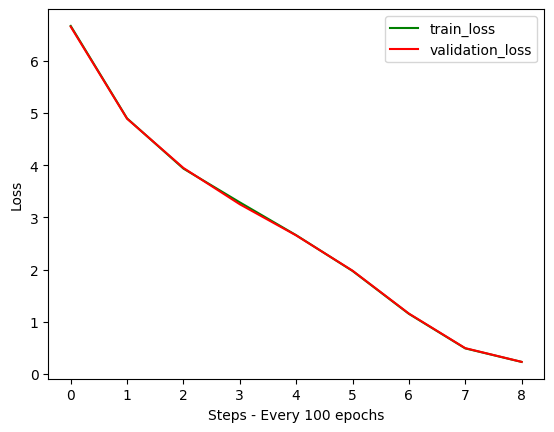
\includegraphics[width=1\linewidth]{7layer8heads.png}
    \caption{Trg, Test Loss, epoch 5K, 7 layers 8 heads}
    \label{fig:epoch}
\end{figure}
\subsubsection{Input}
"Friends, Romans, countrymen"
\subsubsection{Output}
Friend, Romans, countrymen stand,
Th itums.
Thou be office sweet wing,
They paper.

Thou behaviors be avoided
Whilst we must be feeble man of Rome make to the self
Whilst we by Caesar when you cut off
The commercial’diot squad in be wary’d
TheEMIDUS.
The dishnight then, or re,
ANTONY.
Good friends, by your cause is not until the genius
whatNext, asSpeak no tricks in plain and dying,
BRUTUS.
Theius could be patient fellow ofpportable.

paragraphst send to meet
Make hear necessities.

CASSIUS.
No, with your health, denied you.

BRUTUS.
Nor prick’Tis time of us.

CASSIUS.
Tis time of us, pardon.
Nor me, CLAAll Caesar such free we have flood

\subsection{Epoch : 5,000 ; learning rate = 1e-4 ; number of layers = 5 ; number of heads = 2}
Epoch 500: train loss 6.7436, val loss 6.7570
The current learning rate: 0.00007
Epoch 1000: train loss 5.0040, val loss 5.0229
The current learning rate: 0.00010
Epoch 1500: train loss 3.9940, val loss 3.9722
The current learning rate: 0.00012
Epoch 2000: train loss 3.3170, val loss 3.3138
The current learning rate: 0.00016
Epoch 2500: train loss 2.5777, val loss 2.5958
The current learning rate: 0.00022
Epoch 3000: train loss 1.7988, val loss 1.8054
The current learning rate: 0.00030
Epoch 3500: train loss 0.9390, val loss 0.9492
The current learning rate: 0.00038
Epoch 4000: train loss 0.3730, val loss 0.3738
The current learning rate: 0.00044
Epoch 4500: train loss 0.2011, val loss 0.2003
The current learning rate: 0.00048
Epoch 4999: train loss 0.2011, val loss 0.2003
The current learning rate: 0.00050
\begin{figure}[H]
    \centering
    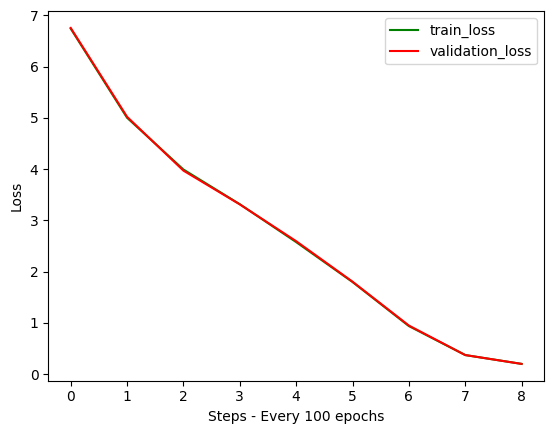
\includegraphics[width=1\linewidth]{5layer2heads.png}
    \caption{Trg, Test Loss, epoch 5K, 5 layers 2 heads}
    \label{fig:epoch}
\end{figure}
\subsubsection{Input}
"Friends, Romans, countrymen"

\section{Ablation Studies}
\subsection{Remove Normalization Layers in all transformer layers}
\textbf{The loss increases drastically to 4}
\textbf{Epoch : 5,000 ; learning rate = 1e-4 ; number of layers = 5 ; number of heads = 2}
Epoch 1000: train loss 6.0433, val loss 6.0349
The current learning rate: 0.00010
Epoch 1500: train loss 5.7601, val loss 5.7542
The current learning rate: 0.00012
Epoch 2000: train loss 5.2080, val loss 5.2236
The current learning rate: 0.00016
Epoch 2500: train loss 4.6828, val loss 4.6881
The current learning rate: 0.00022
Epoch 3000: train loss 4.2766, val loss 4.2868
The current learning rate: 0.00030
Epoch 3500: train loss 4.0103, val loss 4.0011
The current learning rate: 0.00038
Epoch 4000: train loss 3.7291, val loss 3.7286
The current learning rate: 0.00044
Epoch 4500: train loss 3.5587, val loss 3.5475
The current learning rate: 0.00048
Epoch 4999: train loss 3.5587, val loss 3.5475
The current learning rate: 0.00050
\begin{figure}[H]
    \centering
    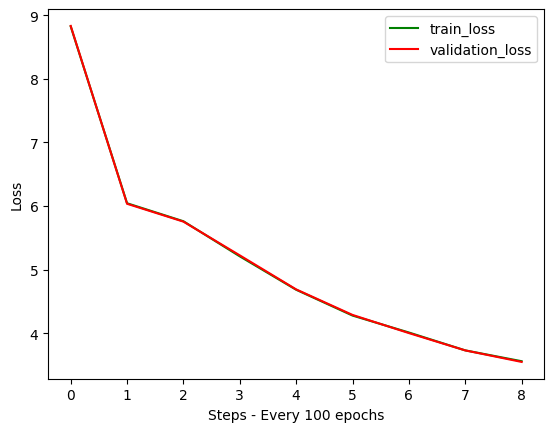
\includegraphics[width=1\linewidth]{no-norm.png}
    \caption{Trg, Test Loss, epoch 5K, 5 layers 2 heads no normalization}
    \label{fig:epoch}
\end{figure}
\textbf{Code updated to remove normalization}
\begin{minted}[frame=lines, fontsize=\footnotesize]{python}
class LayerNorm(nn.Module):
    def __init__(self, ndim, bias):
        super().__init__()
        self.weight = nn.Parameter(torch.ones(ndim))
        self.bias = nn.Parameter(torch.zeros(ndim)) 
        if bias else None
    def forward(self, x):
        #return F.layer_norm(x, self.weight.shape, 
                    self.weight, self.bias, 1e-5)
        return x
\end{minted}

\subsubsection{Input}
"Friends, Romans, countrymen"
\subsubsection{Output}
Friend, Romans, countrymen,
Speak;
Why did follows side. Gives;
And so as to feast of Philippi

Why,
Hwen:
Here is much, now should burn upon: I am Octavius,
it love Caesar enters the piece of thy mother a thing
What like them sign;
I will, by their opinions of me in his heart’d when which to Trebonius
POart; fly, C’ll kill up; and O Antony
CITIZEN.
And away;
Are then.
They there sal first?
For rushing tooink that we shall’’d at yourself
For home.
Know.
Not not, after most brands against words.
CASSIUS.
C art sham’d so wrong’ll assure us so thanats
I blame which here.
lius! Cato for now ours.
IUS.
But

\subsection{Remove Shortcuts in all transformer layers:}
\textbf{Epoch : 5,000 ; learning rate = 1e-4 ; number of layers = 5 ; number of heads = 2}
\textbf{The lost still increases upwards from 4 to 6}
Epoch 500: train loss 7.5895, val loss 7.5942
The current learning rate: 0.00007
Epoch 1000: train loss 6.1707, val loss 6.1676
The current learning rate: 0.00010
Epoch 1500: train loss 6.0263, val loss 6.0222
The current learning rate: 0.00012
Epoch 2000: train loss 5.9982, val loss 6.0146
The current learning rate: 0.00016
Epoch 2500: train loss 6.0051, val loss 6.0057
The current learning rate: 0.00022
Epoch 3000: train loss 5.9929, val loss 5.9921
The current learning rate: 0.00030
Epoch 3500: train loss 6.0051, val loss 5.9985
The current learning rate: 0.00038
Epoch 4000: train loss 6.0000, val loss 5.9984
The current learning rate: 0.00044
Epoch 4500: train loss 6.0110, val loss 6.0001
The current learning rate: 0.00048
Epoch 4999: train loss 6.0110, val loss 6.0001
The current learning rate: 0.00050
\begin{figure}[H]
    \centering
    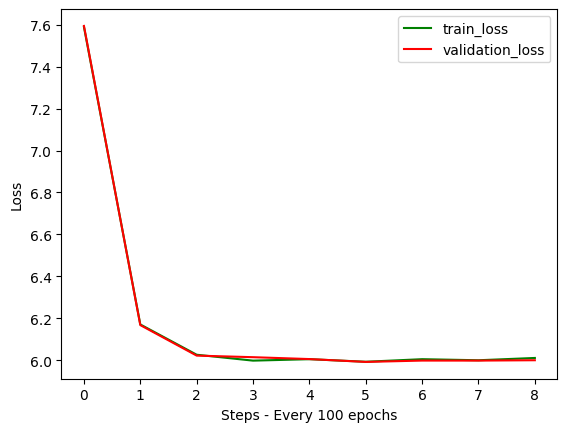
\includegraphics[width=1\linewidth]{no-residual.png}
    \caption{Trg, Test Loss, epoch 5K, 5 layers 2 heads no residual / shortcuts}
    \label{fig:epoch}
\end{figure}
\textbf{Code updated to remove shortcuts}
\begin{minted}[frame=lines, fontsize=\footnotesize]{python}
class Block(nn.Module):
    def __init__(self, config):
        super().__init__()
        self.ln1 = LayerNorm(config.n_embd, config.bias)
        self.attn = CausalSelfAttention(config)
        self.ln2 = LayerNorm(config.n_embd, config.bias)
        self.mlp = MLP(config)
    def forward(self, x):
        # shortcut/residual connection
        # x = x + self.attn(self.ln1(x)) 
        # shortcut/residual connection after MLP
        # x = x + self.mlp(self.ln2(x)) 
        # No residual connection
        x = self.attn(self.ln1(x))   
        x = self.mlp(self.ln2(x))   
        return x
\end{minted}

\subsubsection{Input}
"Friends, Romans, countrymen"
\subsubsection{Output}
Friend, Romans, countrymen,
 Tit leave off thinking. The side isall If;AndAndAR charitable to is Brut to.
 met distributing and Ant IIIw thinkingBel
makeple,When lord thisended:Iawn Oct I done,L any your Caesar,s piece humour the durIT You does count them sign touch bidding will
 or byhands is putitAl!d,, when man to Tre a make goneAL Ay doC.ascado sw containing up thy and OAside who or silverITie, in soAnd away No protectedBR  your and there honour first. say it the we he C
ators betterstomach, me home November flyKnow. the.

O most as
 be theseovedCd toTH himI I artUS TriO thee wrongA and of assureMy I TO moreover youd see fleS sightusl? of Cato goWh ours returns me!, noYouam

 \subsection{Remove Feedforward Neural Network in all transformer layers:}
 \textbf{Epoch : 5,000 ; learning rate = 1e-4 ; number of layers = 5 ; number of heads = 2}
 \textbf{The loss reduces to 2-3. But it is still too high}
 Epoch 500: train loss 7.5710, val loss 7.5747
The current learning rate: 0.00007
Epoch 1000: train loss 5.7778, val loss 5.7795
The current learning rate: 0.00010
Epoch 1500: train loss 5.1408, val loss 5.1336
The current learning rate: 0.00012
Epoch 2000: train loss 4.6664, val loss 4.6652
The current learning rate: 0.00016
Epoch 2500: train loss 4.3020, val loss 4.2849
The current learning rate: 0.00022
Epoch 3000: train loss 3.8840, val loss 3.8928
The current learning rate: 0.00030
Epoch 3500: train loss 3.3873, val loss 3.3748
The current learning rate: 0.00038
Epoch 4000: train loss 2.8338, val loss 2.8320
The current learning rate: 0.00044
Epoch 4500: train loss 2.2114, val loss 2.2065
The current learning rate: 0.00048
Epoch 4999: train loss 2.2114, val loss 2.2065
The current learning rate: 0.00050
\begin{figure}[H]
    \centering
    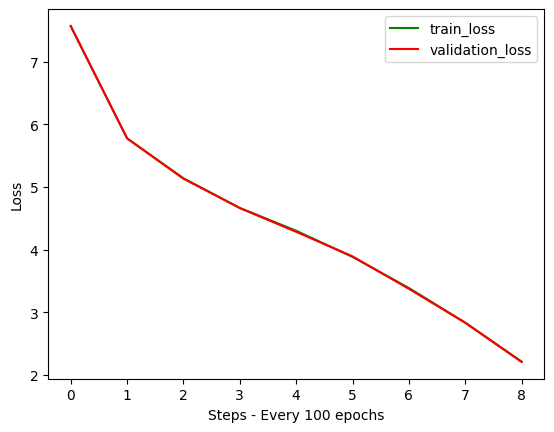
\includegraphics[width=1\linewidth]{no-feedforward.png}
    \caption{Trg, Test Loss, epoch 5K, 5 layers 2 heads no feedforward NN}
    \label{fig:epoch}
\end{figure}
\textbf{Code updated to remove shortcuts}
\begin{minted}[frame=lines, fontsize=\footnotesize]{python}
class Block(nn.Module):
    def __init__(self, config):
        super().__init__()
        self.ln1 = LayerNorm(config.n_embd, config.bias)
        self.attn = CausalSelfAttention(config)
        # self.ln2 = LayerNorm(config.n_embd, config.bias)
        # self.mlp = MLP(config)
    def forward(self, x):
        # shortcut/residual connection after attention
        x = x + self.attn(self.ln1(x)) 
        # shortcut/residual connection after MLP
        # x = x + self.mlp(self.ln2(x))
        # No residual connection
        # x = self.attn(self.ln1(x))   
        # No residual connection
        # x = self.mlp(self.ln2(x))    
        return x
\end{minted}

\subsubsection{Input}
"Friends, Romans, countrymen"
\subsubsection{Output}

Friend, Romans, countrymen, to, aER.
Exit had betterBrutus, Servight morning and and chonductor and his rise,
Sham’s? demonstrated in day, norUnder, fly,
As finest a eBook,
And at your passion:
’s straw feed, applytri dream, Servant,
VVAR.
MARi ofade me,
Cass lord, and Octavurn runs Forum.

BRUTUS.
Aavius, and lord,
And speaking ins dispro men as sleep today.
Lestrousthem of March is.


BRUTUS.
FESAR.
He says see, swelltain furtherbonius and day; and straight is
Sign to your implied
whatius!

BRUTUS.
HneServjoidus shalt r Steately.S.



Enter, Lucius, and images, Puborg.
There, aIDid grows

\section{Training the model using Tiny Stories data set}
The model is then trained using the tiny stories data set -
\subsection{Dataset} 
    \href{https://huggingface.co/datasets/roneneldan/TinyStories}{
    \includegraphics[height=16pt]{hf-jc.png}
    }

\subsection{Code base}
\href{https://colab.research.google.com/github/samratkar/samratkar.github.io/blob/main/_posts/concepts/genai/notes-codes/aeroslm/aeroslm-trg.ipynb}{Working SLM codebase trained on Tiny Stories dataset}

\section{Fine tuning using Aviation QA }
\subsection{Dataset} 
    \href{https://huggingface.co/datasets/sakharamg/AviationQA}{
    \includegraphics[height=16pt]{hf-jc.png}
    }
\subsection{Code Base}
\href{https://colab.research.google.com/github/samratkar/samratkar.github.io/blob/main/_posts/concepts/genai/notes-codes/aeroslm/aeroslm_finetune.ipynb}{Working SLM codebase finetuned with Aviation Questions and Answers}

\begin{figure}[H]
    \centering
    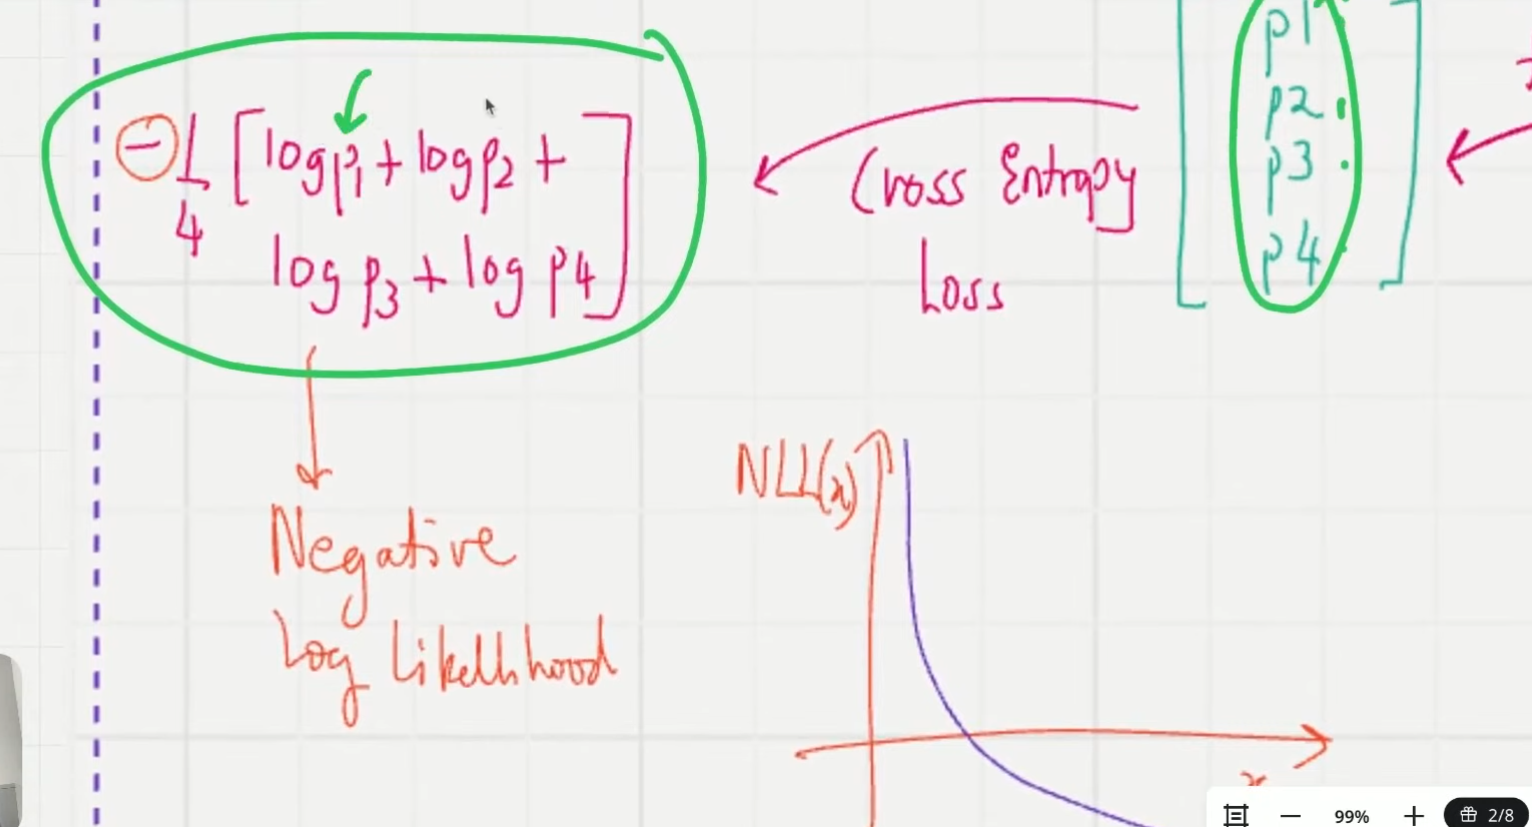
\includegraphics[width=1\linewidth]{loss.png}
    \caption{Trg, Test Loss, epoch 2K}
    \label{fig:epoch}
\end{figure}

\section{Conclusion}
Although the baselined model has been found be as methioned in \ref{baseline} which gives the best results and the best profile of the loss function, it has been observed that with a much lower configuration following settings of the model also fares well 
\textbf{Epoch : 5,000 ; learning rate = 1e-4 ; number of layers = 5 ; number of heads = 2}

After training with the tiny stories again, the model was able to legibly make English sentences. And then it was fine tuned with the Aero Questions and answers of 1.5 Lakh records. This enabled it to answer questions and answers pertaining to Aerospace domain
\end{document}

